\section{Proof of Proposition \ref{prop:gradient_of_m_approximation}}
\label{app:gradient_of_m_approximation}

The Taylor expansion of $\mf{m}(\mf{v})$ at $\mf{v}=\mf{v}^*$ reads
\begin{align}
	\mf{m}(\mf{v}) &= \mf{m}^* + \frac{\partial \mf{m}}{\partial \mf{v}} (\mf{v}-\mf{v}^*) +
	\mathcal{O}_m(\Vert\mf{v}-\mf{v}^*\Vert^2)\nonumber\\
	&=\frac{\partial \mf{m}}{\partial \mf{v}}(\mf{v}-\mf{v}^*) +
	\mathcal{O}_m(\Vert\mf{v}-\mf{v}^*\Vert^2)
	\label{eq:m_taylor_expansion}
\end{align}
where we use the fact that by definition $\mf{m}^*=\mf{m}(\mf{v}^*)=\mf{0}$. All
derivatives are evaluated at $\mf{v} = \mf{v}^*$ unless otherwise noted. We
first evaluate the Jacobian of the mass matrix term in Eq.
(\ref{eq:m_definition})
\begin{align*}
	\frac{\partial \left( \mf{M}(\mf{q}^{\theta_{q}}(\mf{v}))(\mf{v}-\mf{v}_0) \right)}{\partial \mf{v}}
	= \mf{M}(\mf{q}^{\theta_{q}}(\mf{v}^*)) + \mf{E},
\end{align*}
where we defined
\begin{align*}
	\mf{E} = \frac{\partial \mf{M}(\mf{q}^{\theta_{q}})}{\partial\mf{v}} (\mf{v}^*-\mf{v}_0).
\end{align*}
Note that by combining Eqs. (\ref{eq:theta_method}) and (\ref{eq:q_update}), the
mid-step configuration $\mf{q}^{\theta_q}$ can be written as
\begin{align*}
	\mf{q}^{\theta_q}(\mf{v}) &= \mf{q}_0 + dt \theta_q \dot{\mf{q}}^{\theta_{vq}} \\
	                          &= \mf{q}_0 + dt \theta_q \mf{N}(\mf{q}^{\theta_{q}})\mf{v}^{\theta_{vq}}(\mf{v}).
\end{align*}
Hence by the chain rule, $\mf{E}$ can be further calculated as
\begin{align*}
	\mf{E} = dt\theta_q\frac{\partial \mf{M}(\mf{q}^{\theta_{q}}) }{\partial\mf{q}}
             \frac{\partial\dot{\mf{q}}^{\theta_{vq}}}{\partial\mf{v}}
			 (\mf{v}^*-\mf{v}_0).
\end{align*}
Notice that 
\begin{align*}
		\Vert\mf{E}\Vert 
		&\le dt\theta_q \left\| \frac{\partial\mf{M}(\mf{q}^{\theta_{q}})}{\partial\mf{q}}  \right\|
			\left\| \frac{\partial\dot{\mf{q}}^{\theta_{vq}}}{\partial\mf{v}}  \right\|
		    \left\| \mf{v}^*-\mf{v}_0 \right\| \\
		&= \mathcal{O}(dt^2),
\end{align*}
since $\Vert\mf{v}^*-\mf{v}_0\Vert = \mathcal{O}(dt)$.

We proceed similarly to expand the Jacobian of
$\mf{F}(\mf{v})=\mf{F}(\mf{q}^{\theta_{q}}(\mf{v}), \mf{v}^{\theta_v}(\mf{v}))$
as
\begin{align*}
	\frac{\partial\mf{F}}{\partial \mf{v}} = -dt\,\theta_q\theta_{vq}\mf{K}(\mf{q}^{\theta_q},
	\mf{v}^{\theta_v})-\theta_v\mf{D}(\mf{q}^{\theta_q}, \mf{v}^{\theta_v})
\end{align*}
with $\mf{K}$ and $\mf{D}$ the stiffness and damping matrices defined by Eqs.
(\ref{eq:stiffness_matrix})-(\ref{eq:dissipation_matrix}).

We can now write the Jacobian of $\mf{m}(\mf{v})$ in Eq.
(\ref{eq:m_taylor_expansion}) as
\begin{align*}
	\frac{\partial \mf{m}}{\partial \mf{v}} = \mf{A} + \mf{E} - dt\frac{\partial \mf{G}}{\partial \mf{v}}
\end{align*}
where we defined
\begin{align*}
	\mf{A}=\mf{M}+ dt^2\theta_q\theta_{qv}\mf{K}+dt\theta_v\mf{D}.
\end{align*}
With these definitions the Taylor expansion in Eq. (\ref{eq:m_taylor_expansion})
becomes
\begin{align*}
	\frac{\partial\mf{m}}{\partial\mf{v}}(\mf{v}-\mf{v}^*) &= \mf{A}(\mf{v}-\mf{v}^*) + \mf{E}(\mf{v}-\mf{v}^*) \\
	&- dt\frac{\partial\mf{G}}{\partial\mf{v}}(\mf{v}-\mf{v}^*) + \mathcal{O}_m(\Vert\mf{v}-\mf{v}^*\Vert^2).
\end{align*}

Since contact is compliant, forces are finite within the finite interval $\delta
t$ and therefore $\Vert\mf{v}-\mf{v}^*\Vert=\mathcal{O}(dt)$. Thus
\begin{align*}
	\mf{E}(\mf{v}-\mf{v}^*)=\mathcal{O}_E(dt^3), \\
    dt\frac{\partial \mf{G}}{\partial \mf{v}}(\mf{v}-\mf{v}^*)=\mathcal{O}_G(dt^2), \\ 
    \mathcal{O}_m(\Vert\mf{v}-\mf{v}^*\Vert^2) = \mathcal{O}_m(dt^2).
\end{align*}
Therefore, the positive definite linearization
\begin{align*}
	\mf{A}(\mf{v}-\mf{v}^*) + \mathcal{O}_E(dt^3) + \mathcal{O}_G(dt^2) +
	\mathcal{O}_m(dt^2) = \mf{J}^T\mf{\bgamma}
\end{align*}
agrees with the original momentum balance in Eq. (\ref{eq:v_update}) to second
order.

Finally, notice that $\mf{A}$ is a linear combination of positive definite
matrices with non-negative scalars in the linear combination, and therefore
$\mf{A}\succ 0$.\hfill\IEEEQED

\section{Analytical Inverse Dynamics Derivations}
\label{app:analytical_inverse_dynamics_derivations}

\textit{Inverse dynamics} refers to the computation of the impulses given we
know the velocities of the system. It is shown in \cite{bib:todorov2014} that
this problem can be solved analytically given the separable structure of the
constraints. Then the impulse for each $k\text{-th}$ constraint can be solved
from
\begin{eqnarray}
	\bgamma_k&=&
	\begin{aligned}
		\argmin_{\bgamma\in\mathcal{C}} \quad &
	\frac{1}{2}(\bgamma-\mf{y}_k)^T\mf{R}_k(\bgamma-\mf{y}_k) \end{aligned}\\
	\mf{y}_k &=& -\vf{R}_k^{-1}(\mf{v}_{c,k}-\hat{\mf{v}}_{c,k})
\end{eqnarray}

From now on we will omit the index $k$. 

\subsection{Limits}
The solution for limits is trivial since $\mathcal{C}=\mathbb{R}^+$ or a finite
interval. \todo{summrize those results here.}

\subsection{Contact Impulses}

Contact impulses are constrained to the friction cone $\mathcal{C}=\mathcal{F}$.
This problem can be solved using simple geometry by noticing that the change of
variables $\tilde\bgamma=R^{1/2}\bgamma$ (and respectively
$\tilde{\vf{y}}=R^{1/2}\vf{y}$) leads to a projection with Euclidian norm on a
cone $\mathcal{F}_{\tilde\mu}$ with friction coefficient
$\tilde\mu=\mu\,(R_t/R_n)^{1/2}$
\begin{eqnarray}
	P_\mathcal{F_{\tilde\mu}}(\tilde{\vf{y}})&=&\argmin_{\tilde\bgamma\in\mathcal{F_{\tilde\mu}}}
		\quad \frac{1}{2}\Vert\tilde\bgamma-\tilde{\vf{y}}\Vert_2^2\nonumber\\
	P_\mathcal{F}(\vf{y}) &=&
	\vf{R}^{-1/2}P_\mathcal{F_{\tilde\mu}}(\tilde{\vf{y}})
	\label{eq:local_optimization_problem_tilde}
\end{eqnarray}

The optimization problem in the Euclidean norm given by Eq.
(\ref{eq:local_optimization_problem_tilde}) can be solved by inspection. If
$\tilde{\vf{y}}_i\in\tilde{\mathcal{F}}_i$, then we simply have
$\tilde{\bgamma}_i = \tilde{\vf{y}}_i$, we call this \textit{Region I}. If
however $\tilde{\vf{y}}_i$ is inside the negative of the dual cone (a.k.a. the
\textit{polar} cone), the closest point to $\tilde{\vf{y}}_i$ within the (tilde)
friction cone is zero, i.e. $\tilde{\bgamma}_i =\vf{0}$. We call this
\textit{Region III}. Finally, if $\tilde{\vf{y}}_i$ is in the region outside
both $\tilde{\mathcal{F}}_i$ and its polar $\tilde{\mathcal{F}}_i^\circ$, then
the closest point is it's Euclidian projection on the boundary of
$\tilde{\mathcal{F}}_i$. We call this \textit{Region II}. Figure
\ref{fig:cone_regions} shows a schematic of $\tilde{\mathcal{F}}_i$,
$\tilde{\mathcal{F}}_i^\circ$ and labels the three different regions. From Fig.
\ref{fig:cone_regions}, for a cone forming an angle $\theta$ with the z axis, we
have $\tan(\theta)=\tilde\mu$ and $\cos(\theta)=1/(1+\tilde\mu^2)$. Then the
projection can be written as
\begin{eqnarray}
	\tilde{\bgamma}_t &=& \tilde{\mu}\tilde{\gamma}_n\hat{\vf{t}}\nonumber\\
	\tilde{\gamma}_n &=& \frac{1}{1+\tilde{\mu}^2}\left(\tilde{y}_n +
	\tilde{\mu}\tilde{y}_r\right)\nonumber		
\end{eqnarray}
where $\tilde\mu=\mu(R_t/R_n)^{1/2}$ and the tangent vector is defined as
$\hat{\vf{t}}=\vf{y}_t/\Vert\vf{y}_t\Vert=-\vf{v}_t/\Vert\vf{v}_t\Vert$. 
\begin{figure}[!h]
    \centering
    %\vspace{6pt}
    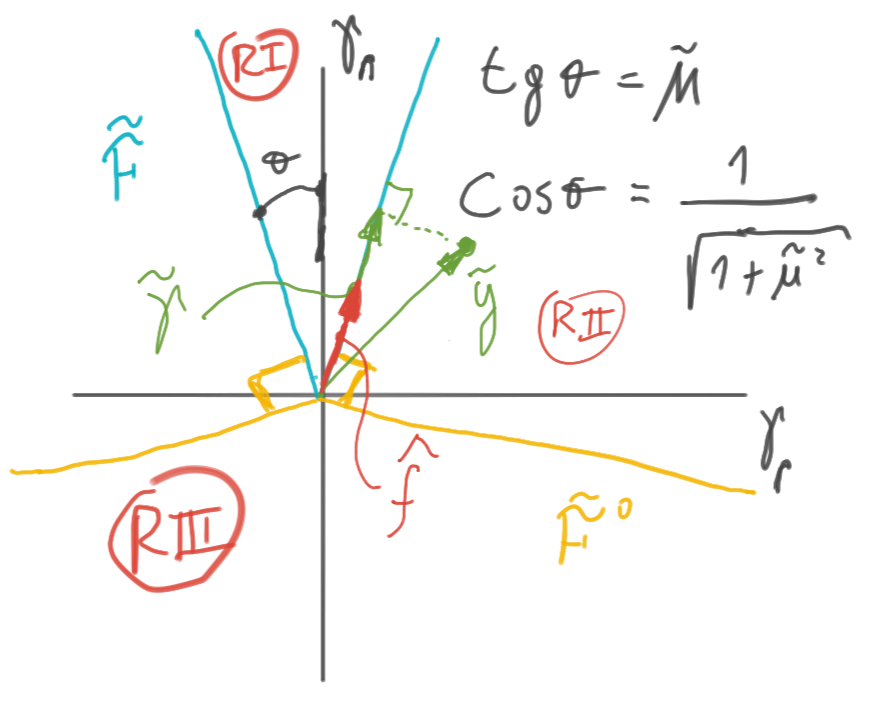
\includegraphics[width=0.45\columnwidth]{figures/cone_regions.png}
    \caption{Geometry of $\tilde{\mathcal{F}}_i$ and regions in the
    $\tilde{\vf{y}}$ space.}
    \label{fig:cone_regions}
\end{figure}

The desired expression for the original impulses
$\bgamma=\mf{R}^{-1/2}\tilde\bgamma$ in Region II is
\begin{eqnarray}
	\bgamma_t &=& \mu\gamma_n\hat{\vf{t}}\nonumber\\
	\gamma_n &=& \frac{1}{1+\tilde\mu^2}\left(y_n +
	\mu\frac{R_t}{R_n}y_r\right)\nonumber		
\end{eqnarray}

Finally, we can write the an analytical expression for $P_\mathcal{F}$ as
\begin{equation}
	\bgamma = P_\mathcal{F}(\vf{y}) = 
\begin{dcases}
	% Region I, stiction
	\vf{y} 
	% When we  have:
	& \text{stiction, } y_r < \mu y_n\\
	%
	%
	% Region II, sliding.
	\begin{bmatrix}
		\mu\gamma_n\hat{\vf{t}}\\
		\frac{1}{1+\tilde\mu^2}\left(y_n +
	\mu\frac{R_t}{R_n}y_r\right)
	\end{bmatrix}
	% When we  have:
	& \text{sliding, } -\mu \frac{R_t}{R_n} y_r < y_n \leq \frac{y_r}{\mu}\\
	%
	%
	% Region III, no contact.
    \vf{0} & \text{no contact, } y_n \leq -\mu \frac{R_t}{R_n} y_r
\end{dcases}	  
	\label{eq:inverse_dynamics_projection}
\end{equation}
where $\vf{y}_t$ and $y_n$ are the tangential and normal components of $\vf{y}$,
the radial component is defined as $y_r=\Vert\vf{y}_t\Vert$ and the tangent
vector as $\hat{\vf{t}}=\vf{y}_t/y_r$. We also defined the common dimensionless
factors $\tilde\mu=\mu\,(R_t/R_n)^{1/2}$ and $\hat\mu=\mu\,R_t/R_n$.


\section{Proof of Theorem \ref{th:unconstrained_formulation_equivalance}}
\label{app:unconstrained_formulation_equivalance}
Before proving this theorem, we need the following result.
\begin{lemma}
    The conic constraint $\mf{g}(\mf{v}, \bsigma)\in\mathcal{F}^*$ is satisfied
    if $\bsigma$ is given by $P_\mathcal{F}(\mf{y(\mf{v})})$.
    \label{lemma:conic_constraints_are_satisfied_analytically}
\end{lemma}
\begin{IEEEproof}
    Since $\bsigma$ is the projection of $\mf{y}(\mf{v})$ to the cone
    $\mathcal{F}$ with the $\mf{R}$ norm, by Moreau's decomposition theorem, we
    know that $\mf{y}(\mf{v}) - \bsigma$ is in the polar cone of $\mathcal{F}$
    with the $\mf{R}$ norm. That is,
    \begin{align*}
        \langle \mf{y}(\mf{v}) - \bsigma, \mf{x} \rangle_\mf{R} \le 0 
    \end{align*}
    for all $\mf{x} \in \mathcal{F}$, with the inner product
    $\langle\mf{v},\mf{w}\rangle_\mf{R}=\mf{v}^T\mf{R}\mf{w}$. Reorganizing
    terms, we get
    \begin{align*}
        \mf{x}^T \mf{R}(\mf{y}(\mf{v}) - \bsigma) &\le 0 \\
        \mf{x}^T (-\mf{R}\bsigma - \mf{v}_c + \hat{\mf{v}}_c) &\le 0 \\
        \langle \mf{x}, -\mf{R}\bsigma - \mf{v}_c + \hat{\mf{v}}_c \rangle &\le 0
    \end{align*}
    for all $\mf{x} \in \mathcal{F}$. Therefore, it follows that
    $-\mf{g}=-(\mf{v}_c - \hat{\mf{v}}_c + \mf{R}\bsigma)$ is in the polar cone
    of $\mathcal{F}$ and thus $\mf{g}$ is in the dual cone of $\mathcal{F}$.
\end{IEEEproof}

The optimality condition for the unconstrained formulation in
\eqref{eq:primal_unconstrained} is $\nabla\ell_p(\mf{v})=\mf{0}$. It is shown in
Appendix \ref{app:gradients_derivation} that
\begin{equation*}
    \nabla\ell_p(\mf{v})=\mf{A}(\mf{v}-\mf{v}^*) - \mf{J}^T\bgamma(\mf{v})
\end{equation*}
\RedHighlight{TODO: Make sure the appendix is consistent when you update it. In
particular, the appendix has $\mf{M}$ instead of $\mf{A}$.} with impulses given
by $\bgamma(\mf{v})=P_\mathcal{F}(\mf{y}(\mf{v}))$, the dual optimal. Therefore,
$\nabla\ell_p(\mf{v})=\mf{0}$ implies \eqref{eq:momentum_optimality}, the first
optimality condition for \eqref{eq:primal_regularized}.
   
The analytical inverse dynamics solution shows that $\bgamma =
P_\mathcal{F}(\mf{y(\mf{v})})$ with the primal optimal $\mf{v}$. Hence, choosing
$\bsigma = P_\mathcal{F}(\mf{y(\mf{v})})$ with the primal optimal $\mf{v}$
satisfies \eqref{eq:sigma_equal_gamma}, the second optimality condition for
\eqref{eq:primal_regularized}.

Finally, by Lemma \ref{lemma:conic_constraints_are_satisfied_analytically}, the
cone constraint $\mf{g}(\mf{v}, \bsigma)\in\mathcal{F}^*$ is satisfied.
\hfill\IEEEQED


\section{Derivation of the Gradients}
\label{app:gradients_derivation}

We first compute the regularization term as
\begin{eqnarray}
	\ell_R = \frac{1}{2}(R_t\Vert\bgamma_t\Vert^2+R_n\gamma_n^2)
\end{eqnarray}

During \textbf{stiction} the cost is written as
\begin{eqnarray}
	\ell_R(\vf{y}) = \frac{1}{2}(R_t y_r^2+R_n y_n^2)
\end{eqnarray}

During \textbf{sliding} Eq. (\ref{eq:inverse_dynamics_projection}) applies and
the cost can be written as
\begin{eqnarray}
	\ell_R(\vf{y}) =
	\frac{1}{2}\gamma_n^2(R_t\mu^2+R_n)=\frac{R_n}{2}(1+\tilde\mu^2)\gamma_n^2=\frac{R_n}{2(1+\tilde\mu^2)}\left(\mu\frac{R_t}{R_n}y_r+y_n\right)^2
\end{eqnarray}

and finally when there is \textbf{no contact}
\begin{eqnarray}
	\ell_R(\vf{y}) = 0
\end{eqnarray}

Therefore $\ell_R$ is a piecewise function that we can summarize as
\begin{equation}
	\ell_R(\vf{y}) = 
\begin{dcases}
	% Region I, stiction
	\frac{1}{2}(R_t y_r^2+R_n y_n^2) & \text{stiction, } y_r < \mu y_n\\
	% Region II, sliding.
	\frac{R_n}{2(1+\tilde\mu^2)}\left(\mu\frac{R_t}{R_n}y_r+y_n\right)^2 & \text{sliding, } -\mu \frac{R_t}{R_n} y_r < y_n \leq \frac{y_r}{\mu}\\
	% Region II, no contact.
    \vf{0} & \text{no contact, } y_n \leq -\mu \frac{R_t}{R_n} y_r
\end{dcases}	  
	\label{eq:ell_R_piecewise}
\end{equation}

\subsection{Gradients per Contact Point}
In this section we compute the gradients of $\ell_R(\mf{y})$ with respect to the
$i\text{-th}$ contact point variable $\vf{y}_i\in\mathbb{R}^3$. Unless otherwise
stated, in this section we'll drop the subindex $i$ for the $i\text{-th}$
contact point. Therore in this section $\nabla_\vf{y}\ell_R\in\mathbb{R}^3$ and
$\nabla_\vf{y}^2\ell_R\in\mathbb{R}^{3\times 3}$ (notice that as per our
notation, we consistently use a bold italic font for 3D vectors and only bold,
not italic, for $n\text{-dimensional}$ vectors.)

The full gradient $\nabla_\mf{y}\ell_R$ concatenates the three-dimensional
gradients $\nabla_\vf{y}\ell_R$ while the full Hessian matrix is block-diagonal
with each $3\times 3$ block containing the local $i\text{-th}$ point Hessian.
This is particularly useful to exploit sparsity in the computations.

We use the following identities to simplify the expressions
\begin{eqnarray}
	\frac{\partial y_r}{\partial\vf{y}_t} &=& \hat{\vf{t}}\nonumber\\
	\frac{\partial \hat{\vf{t}}}{\partial\vf{y}_t} &=&
	\frac{\vf{P}^\perp(\hat{\vf{t}})}{y_r}
	\label{eq:yt_derivatives}
\end{eqnarray}
where the $2\times 2$ projection matrices along and perpendicular to
$\hat{\vf{t}}$ are defined as
\begin{eqnarray}
	\vf{P}(\hat{\vf{t}}) &=& \hat{\vf{t}}\otimes\hat{\vf{t}}\nonumber\\
	\vf{P}^\perp(\hat{\vf{t}})&=&\vf{I}_2 - \vf{P}(\hat{\vf{t}})
	\label{eq:tangential_projections}
\end{eqnarray}

Taking the gradient of Eq. (\ref{eq:ell_R_piecewise}) results in
\begin{equation}
	\nabla_\vf{y}\ell_R(\vf{y}) = 
\begin{dcases}
	%%%%%%%%%%%%%%%%%%%%
	% Region I, stiction
	\vf{R}\,\vf{y} & 
	% when,
	\text{stiction, } y_r < \mu y_n\\
	%
	%%%%%%%%%%%%%%%%%%%%
	% Region II, sliding.
	\frac{1}{1+\tilde\mu^2}\hat{s}^\circ(\vf{y})\begin{bmatrix}
		\mu R_t\hat{\vf{t}}\\
		R_n\\
	\end{bmatrix} &
	% when,
	\text{sliding, } -\mu \frac{R_t}{R_n} y_r < y_n \leq \frac{y_r}{\mu}\\
	% Region II, no contact.
    \vf{0} & \text{no contact, } y_n \leq -\mu \frac{R_t}{R_n} y_r
\end{dcases}	  
	\label{eq:gradient_ell_R_piecewise}
\end{equation}
where we defined $\hat{\mu}=\mu R_t/R_n$ and $\hat{s}^\circ(\vf{y}) =
\hat{\mu}y_r+y_n$. $\hat{s}^\circ(\vf{y})$ is a measure how close the solution
is to the polar cone $\mathcal{F}^\circ$. $\hat{s}^\circ(\vf{y}) > 0$ in the
sliding region and $\hat{s}^\circ<0$ when there is no contact.

Similarly, we can compute the Hessian of $\ell_R$ by taking the gradient in Eq.
(\ref{eq:gradient_ell_R_piecewise})
\begin{equation}
	\nabla_\vf{y}^2\ell_R(\vf{y}) = 
\begin{dcases}
	%%%%%%%%%%%%%%%%%%%%
	% Region I, stiction
	\vf{R} & 
	% when,
	\text{stiction, } y_r < \mu y_n\\
	%
	%%%%%%%%%%%%%%%%%%%%
	% Region II, sliding.
	\frac{R_n}{1+\tilde\mu^2}
	\begin{bmatrix}
		% ∂²ℓ/∂yₜ²:
		\hat{\mu}\left(\hat{\mu}\vf{P}(\hat{\vf{t}})+\hat{s}^\circ(\vf{y})\vf{P}^\perp(\hat{\vf{t}})/y_r\right) & 
		% ∂²ℓ/∂yₙ∂yₜ:
		\hat{\mu}\vf{t}\\
		% ∂²ℓ/∂yₜ∂yₙ:
		\hat{\mu}\vf{t}^T & 
		% ∂²ℓ/∂yₙ²:
		1\\
	\end{bmatrix} &
	% when,
	\text{sliding, } -\mu \frac{R_t}{R_n} y_r < y_n \leq \frac{y_r}{\mu}\\
	% Region II, no contact.
    \vf{0} & \text{no contact, } y_n \leq -\mu \frac{R_t}{R_n} y_r
\end{dcases}	  
	\label{eq:hessian_ell_R_piecewise}
\end{equation}

Clearly in the stiction region we have $\nabla_\vf{y}^2\ell_R(\vf{y})\succ 0$.
Since in the stiction region we have $\hat{s}^\circ(\vf{y})>0$, the linear
combination of $\vf{P}(\hat{\vf{t}})$ and $\vf{P}(\hat{\vf{t}})^\perp$ in Eq.
(\ref{eq:hessian_ell_R_piecewise}) is PSD (since both projection matrices are
PSD). Therefore, in the sliding region we find out that
$\nabla_\vf{y}^2\ell_R(\vf{y})\succeq 0$.
\todo{Show that the jump condition across the cone's boundary is satisfied.}

\subsection{Gradients with Respect to Velocities}
These gradients are computed using the chain rule since we know that
\begin{equation}
	\mf{y}=\mf{Jv+b}
\end{equation}

The gradient is
\begin{equation}
	\nabla_\mf{v}\ell_R = -\mf{J}^T\mf{R}^{-1}\nabla_\mf{y}\ell_R
	\label{eq:ell_velocity_gradient}
\end{equation}
which, using Eq. (\ref{eq:gradient_ell_R_piecewise}), can be written as
\begin{equation}
	\nabla_\mf{v}\ell_R = -\mf{J}^T\bgamma
	\label{eq:ell_velocity_gradient_simplified}
\end{equation}

And the Hessian is
\begin{equation}
	\nabla_\mf{v}^2\ell_R = \mf{J}^T\mf{R}^{-1}\nabla_\mf{y}^2\ell_R\mf{R}^{-1}\mf{J}
	\label{eq:ell_velocity_hessian}
\end{equation}

Since we already showed $\nabla_\mf{y}^2\ell_R\succeq 0$, it follows that
$\nabla_\mf{v}^2\ell_R\succeq 0$. Therefore the cost $\ell_R(\mf{v})$ is convex.

Recall that $\nabla_\mf{y}^2\ell_R$ is block diagonal and $\mf{R}$ is diagonal.
Therefore the Hessian $\nabla_\mf{v}^2\ell_R$ inherits the same sparsity
structure as the product $\mf{J}^T\mf{J}$.

\subsection{Gradients of the Primal Cost}
With these results, we can now write the gradient and Hessian of the primal cost
$\ell_p(\mf{v})$ in Eq. (\ref{eq:primal_unconstrained}). For the gradient we
have
\begin{equation}
	\nabla_\mf{v}\ell_p(\mf{v}) = \mf{M}(\mf{v}-\mf{v}^*) + \nabla_\mf{v}\ell_R
\end{equation}

Notice that, using Eq. (\ref{eq:ell_velocity_gradient_simplified}), the gradient
can be written as
\begin{equation}
	\nabla_\mf{v}\ell_p(\mf{v}) = \mf{M}(\mf{v}-\mf{v}^*) - \mf{J}^T\bgamma
\end{equation}
and since the unconstrained minimization looks for $\nabla_\mf{v}\ell_p=\mf{0}$,
we essentially recover the balance of momentum, as expected.

Similarly, we can write the Hessian as
\begin{equation}
	\mf{H} = \nabla_\mf{v}^2\ell_p(\mf{v}) = \mf{M} + \nabla_\mf{v}^2\ell_R
\end{equation}
and since we already proved that $\nabla_\mf{v}^2\ell_R\succeq 0$, we find that
the $\nabla_\mf{v}^2\ell_p\succ 0$. Therefore $\ell_p(\mf{v})$ is strictly
convex and there is a unique solution to the minimization problems in the
velocities $\mf{v}$.

\section{More on Projections and the Expanded Sparse System}
\label{app:more_on_projections}
\RedHighlight{See where to put these. Super important. For now I'll place them
here cause I don't wanna forget.}

The Euclidean projection $P_{\mathcal{F}_{\tilde{\mu}}}$ can be written as
	\begin{equation}
		\tilde{\bgamma} = P_{\mathcal{F}_{\tilde{\mu}}}(\tilde{\vf{y}}) = 
	\begin{dcases}
		% Region I, stiction
		\tilde{\vf{y}}
		% When we  have:
		& \text{stiction, } \tilde{y}_r < \tilde{\mu} \tilde{y}_n\\
		%
		%
		% Region II, sliding.
		\begin{bmatrix}
			\tilde{\mu}\tilde{\gamma}_n\hat{\vf{t}}\\
			\frac{1}{1+\tilde\mu^2}\left(\tilde{y}_n +
		\tilde\mu\tilde{y}_r\right)
		\end{bmatrix}
		% When we  have:
		& \text{sliding, } -\tilde\mu \tilde{y}_r < \tilde{y}_n \leq \tilde{y}_r/\tilde\mu\\
		%
		%
		% Region III, no contact.
		\vf{0} & \text{no contact, } \tilde{y}_n \leq -\tilde\mu\tilde{y}_r
	\end{dcases}	  
		\label{eq:projection_tilde}
	\end{equation}
	
With the help of the Eqs.
(\ref{eq:yt_derivatives})-(\ref{eq:tangential_projections}) the gradient can be
computed directly from Eq. (\ref{eq:projection_tilde})

\begin{equation}
	\sGtilde = 
	\begin{dcases}
		% Region I, stiction
		\mf{I}_3
		% When we  have:
		& \text{stiction, } \tilde{y}_r < \tilde{\mu} \tilde{y}_n\\
		%
		%
		% Region II, sliding.
		\frac{1}{1+\tilde\mu^2}
		\begin{bmatrix}
			\tilde\mu^2\mf{P} & \tilde\mu\sthat\\
			\tilde\mu\sthat^T & 1
		\end{bmatrix} +
		\frac{\tilde\mu\tilde\gamma_n}{\tilde{y}_r}
		\begin{bmatrix}
			\mf{P}^\perp & \mf{0}\\
			\mf{0} & 0
		\end{bmatrix}
		% When we  have:
		& \text{sliding, } -\tilde\mu \tilde{y}_r < \tilde{y}_n \leq \tilde{y}_r/\tilde\mu\\
		%
		%
		% Region III, no contact.
		\mf{0}_3 & \text{no contact, } \tilde{y}_n \leq -\tilde\mu\tilde{y}_r
	\end{dcases}
	\label{eq:Gtilde}
\end{equation}
We will show below that $\sGtilde\succeq 0$ even in the sliding regime.

\begin{lemma}
In the sliding region, the gradient $\sGtilde$ can be decomposed as the linear
combination of two projections.
\end{lemma}
\begin{proof}
We write Eq. (\ref{eq:Gtilde}) as
	\begin{equation}
		\sGtilde = \mf{P}_1 + \lambda_3 \mf{P}_3
	\end{equation}	
	where
	\begin{eqnarray}
		\mf{P}_1 &=& 
		\frac{1}{1+\tilde\mu^2}
			\begin{bmatrix}
				\tilde\mu^2\mf{P} & \tilde\mu\sthat\\
				\tilde\mu\sthat^T & 1 \end{bmatrix}\\
		\mf{P}_3 &=& 		
			\begin{bmatrix}
				\mf{P}^\perp & \mf{0}\\
				\mf{0} & 0
			\end{bmatrix}
	\end{eqnarray}
are orthogonal projections along directions $\vf{v}_1$ and $\vf{v}_3$
respectively with
\begin{eqnarray}
	% First
	\vf{v}_1 =& \frac{1}{(1+\tilde\mu^2)^{1/2}}
	\begin{bmatrix}
		\tilde\mu\sthat\\
		1 \end{bmatrix},\\
	%
	% Third
	\vf{v}_3 =& 
	\begin{bmatrix}
		\sthat^\perp\\
		0 \end{bmatrix},
\end{eqnarray}
and $\lambda_3 = \tilde\mu\tilde\gamma_n/\tilde{y}_r$.
\end{proof}
		
%%%%%%%%%%%%%%%%%%%%%%%%%%%%%%%%%%%%%%%%%%%%%%%%%%%%%%%%%%%%%%%%%%%%%%%%%%%%%%%%
%%%%%%%%%%%%%%%%%%%%%%%%%%%%%%%%%%%%%%%%%%%%%%%%%%%%%%%%%%%%%%%%%%%%%%%%%%%%%%%%

\begin{theorem}
During sliding, the eigenvectors $\vf{v}_i$ and eigenvalues $\lambda_i$ of
$\sGtilde$ are
\begin{eqnarray}
	% First
	\vf{v}_1 =& \frac{1}{(1+\tilde\mu^2)^{1/2}}
	\begin{bmatrix}
		\tilde\mu\sthat\\
		1 \end{bmatrix},&\quad\lambda_1 = 1\nonumber\\
	%
	% Second
	\vf{v}_2 =& \frac{1}{(1+\tilde\mu^2)^{1/2}}
	\begin{bmatrix}
		\sthat\\
		-\tilde\mu \end{bmatrix},&\quad\lambda_2 = 0\nonumber\\
	%
	% Third
	\vf{v}_3 =& 
	\begin{bmatrix}
		\sthat^\perp\\
		0 \end{bmatrix},&\quad\lambda_3 =
	\frac{\tilde\mu\tilde\gamma_n}{\tilde{y}_r}
	\label{eq:Gtilde_eigenvectors}
\end{eqnarray}
\end{theorem}
\begin{proof}
We can prove this theorem geometrically. Notice that $\vf{v}_1$ is a vector
along the wall of the cone. Geometrically, projections of vectors lying on the
wall of the cone should give the same vector, and thus $\lambda_1=1$. On the
ohter hand $\vf{v}_2$ is a vector perpendicular to the wall of the cone.
Therefore its proejction is zero, and thus $\lambda_2=0$. Finally, notice
$\vf{v}_3 = \vf{v}_1\times\vf{v}_2$ is a vector tangent to the circumference of
the cone for a fixed $\tilde\gamma_n$. Infinitesimal variations along this
direction at a radial distance $\tilde{y}_r$ project onto the wall of the cone
with radius $\tilde\mu\tilde\gamma_n$, therefore
$\lambda_3=\tilde\mu\tilde\gamma_n/\tilde{y}_r$.

We can verify that indeed $\sGtilde\vf{v}_i=\lambda_i\vf{v}_i$ algebraically.
\end{proof}
\begin{corollary}
$\sGtilde$ is positive semi-definite.
\end{corollary}
\begin{proof}
In the stiction and no-contact regions this is trivially true. In the sliding
region we use the fact that eigenvalues $\lambda_i$ are always positive.
\end{proof}

%%%%%%%%%%%%%%%%%%%%%%%%%%%%%%%%%%%%%%%%%%%%%%%%%%%%%%%%%%%%%%%%%%%%%%%%%%%%%%%%
%%%%%%%%%%%%%%%%%%%%%%%%%%%%%%%%%%%%%%%%%%%%%%%%%%%%%%%%%%%%%%%%%%%%%%%%%%%%%%%%

\begin{theorem}
	The gradient of the regularizer can be written as
	\begin{equation}
		\nabla_\mf{v}\ell_R = -\mf{J}^T\bgamma
		\label{eq:ellR_gradient}
	\end{equation}
\end{theorem}
\begin{proof}
	I believe you can simply use the optimality conditions of the primal for a
	much simpler and cleaner proof. No need to go through cumbersome
	algebra?\todo{do this.}
\end{proof}

\begin{lemma}
	Using the chain rule we can prove that $\mf{G} = \nabla_{\vf{y}}\bgamma =
	\ssqrtRinv\sGtilde\ssqrtR$.
	\label{lemma:PPtilde}
\end{lemma}

%%%%%%%%%%%%%%%%%%%%%%%%%%%%%%%%%%%%%%%%%%%%%%%%%%%%%%%%%%%%%%%%%%%%%%%%%%%%%%%%
%%%%%%%%%%%%%%%%%%%%%%%%%%%%%%%%%%%%%%%%%%%%%%%%%%%%%%%%%%%%%%%%%%%%%%%%%%%%%%%%

Lemma \ref{lemma:PPtilde} will help us proof the following theorem.
\begin{theorem}
	The Hessian of the regularizer can be written as
	\begin{equation}
		\nabla_\mf{v}^2\ell_R = \sJT\ssqrtRinv\,\sGtilde\,\ssqrtRinv\sJ
		\label{eq:ellR_hessian_from_Ptilde}
	\end{equation}
\end{theorem}
\begin{corollary}
	$\nabla_\mf{v}^2\ell_R\succeq 0 $ since $\sGtilde \succeq 0$.
\end{corollary}
\begin{proof}
This simply entails using the chain rule in Eq. (\ref{eq:ellR_gradient}) 
\begin{eqnarray}
	\mf{H}_R = \nabla_\mf{v}^2\ell_R &=& -\sJT
	\nabla_{\vf{v}_c}\bgamma\,\sJ\nonumber\\
	&=&-\sJT \nabla_{\vf{y}}\bgamma\nabla_{\vf{v}_c}\vf{y}\,\sJ\nonumber\\
	&=&\sJT \nabla_{\vf{y}}\bgamma\sRinv\,\sJ
\end{eqnarray}
and substitution of the result in Lemma \ref{lemma:PPtilde} allows us to obtain
 Eq. (\ref{eq:ellR_hessian_from_Ptilde}).
\end{proof} 

%%%%%%%%%%%%%%%%%%%%%%%%%%%%%%%%%%%%%%%%%%%%%%%%%%%%%%%%%%%%%%%%%%%%%%%%%%%%%%%%
%%%%%%%%%%%%%%%%%%%%%%%%%%%%%%%%%%%%%%%%%%%%%%%%%%%%%%%%%%%%%%%%%%%%%%%%%%%%%%%%

\begin{theorem}
The root square of gradient $\sGtilde$ is 
\begin{equation}
	\sGtilde^{1/2} = \mf{P}_1 + \lambda_3^{1/2}\mf{P}_3
\end{equation}
\end{theorem}
\begin{proof}
The eigenvectors of $\sGtilde$ form an orthonormal basis of $\mathbb{R}^3$ and
therefore we can diagonalize $\sGtilde$ via an orthogonal transformation. In
this case, we can write the root square as
\begin{equation}
	\sGtilde = \sum_{i=1}^{3} \lambda_i\vf{v}_i\otimes\vf{v}_i
	\label{eq:toot_square_from_eigenvalues}
\end{equation}
Direct substitution of Eq. (\ref{eq:Gtilde_eigenvectors}) into Eq.
(\ref{eq:toot_square_from_eigenvalues}) completes the proof.
\end{proof}


%%%%%%%%%%%%%%%%%%%%%%%%%%%%%%%%%%%%%%%%%%%%%%%%%%%%%%%%%%%%%%%%%%%%%%%%%%%%%%%%
%%%%%%%%%%%%%%%%%%%%%%%%%%%%%%%%%%%%%%%%%%%%%%%%%%%%%%%%%%%%%%%%%%%%%%%%%%%%%%%%


\begin{theorem}
We can write the Hessian of the regularizer as
\begin{equation}
	\mf{H}_R=\sJbarT\sJbar
\end{equation}
where $\sJbar=\sB\,\sJ$ and $\sB = \sGtilde^{1/2}\,\ssqrtRinv$.
\end{theorem} 
\begin{proof}
We use substitute $\sGtilde=\sGtilde^{1/2}\sGtilde^{1/2}$ in Eq.
(\ref{eq:ellR_hessian_from_Ptilde}) to write
\begin{eqnarray}
	\nabla_\mf{v}^2\ell_R &=&
	\sJT\ssqrtRinv\,\sGtilde^{1/2}\,\sGtilde^{1/2}\,\ssqrtRinv\sJ\nonumber\\
	&=& (\sGtilde^{1/2}\,\ssqrtRinv\sJ)^T\,(\sGtilde^{1/2}\,\ssqrtRinv\sJ)
\end{eqnarray}
where we used the fact that both $\sGtilde^{1/2}$ and $\ssqrtRinv$ are both
symmetric.
\end{proof}

\subsection{The Expanded System}
If we define $\Delta\mf{z}=-\sJbar\Delta\mf{dv}$ we can write the original
Newton iteration from Eq. (\ref{eq:Newton_iteration}) in expanded form as
\begin{eqnarray}
	\begin{bmatrix}
		\sM & -\sJbarT\\
		\sJbar & \mf{I}
	\end{bmatrix}
	\begin{bmatrix}
		\Delta\mf{v}\\
		\Delta\mf{z} \end{bmatrix}=
	\begin{bmatrix}
		-\nabla_\mf{v}\ell_p\\
		\mf{0}
	\end{bmatrix}	
\end{eqnarray}
